\section{Realisatie}
In \cref{sec:ontwerp} is voor elk onderdeel van het systeem besproken wat de eisen zijn van dat onderdeel. Dit hoofdstuk gaat in op de implementatie van elk van deze systeemonderdelen.

\subsection{Spanningsreferentie}
Zoals besproken in \cref{sec:referenceVoltage} kunnen de weerstandswaardes van de spanningsreferentie erg hoog gekozen worden. Met een $R_1$ van \qty{5.6}{\mega\ohm} gebruikt de spanningsdeler \qty{1.65}{\micro\watt}.

Volgens \cref{eq:dividerNoise} heeft de condensatorwaarde wel effect op de ruis. Met een condensator van \qty{1}{\micro\farad} produceert de spanningsreferentie \qty{64.4}{\nano\volt} aan ruis. Dit zorgt voor een signaal-ruis verhouding van \qty{138}{\decibel}, wat meer dan genoeg is.

Deze gekozen waardes en de resulterende eigenschappen zijn te vinden in \cref{tab:divider}.

\begin{table}[ht]
\centering
\begin{tabular}{l|l|l}
    Symbool & Waarde & Eenheid \\
    \hline
    $R_1$       & 5.6  & $\si{\mega\ohm}$   \\
    $R_2$       & 1.0  & $\si{\mega\ohm}$   \\
    $C$         & 1.0  & $\si{\micro\farad}$\\
    $P$         & 1.65 & $\si{\micro\watt}$ \\
    $u_{n,out}$ & 64.4 & $\si{\nano\volt}$  \\
    SNR         & 138  & $\si{\decibel}$
\end{tabular}
\caption{De gekozen waardes van de spanningsdeler, met het resulterende vermogensverbruik en de ruiseigenschappen.}
\label{tab:divider}
\end{table}


\subsection{Microcontroller}
Het digitale gedeelte van het energieverbruik kan opgedeeld worden in 3 onderdelen: de ADC, de digitale signaalverwerking (\cref{fig:digitaleBewerkingsFunctie}) en het draadloos versturen van data. Het is mogelijk om elk van deze onderdelen met aparte componenten te implementeren. Er zijn echter ook componenten beschikbaar die al over elk van deze functionaliteiten beschikken.

Een voorbeeld van een dergelijk component is de nRF52810. Deze microcontroller beschikt over meerdere 14 bit ADC kanalen\footnote{De ADC kanalen zijn alleen 14 bit met oversampling.} en een ingebouwde 2.4GHz Bluetooth transceiver. 
Ook heeft de microcontroller een slaapstand die onderbroken kan worden door een ingebouwde RTC, wat nuttig is voor het periodiek samplen en versturen van pH waardes. In deze slaapstand wordt er zo'n \qty{1.5}{\micro\ampere} gebruikt. Met een voedingsspanning van \qty{3.3}{\volt} komt dit uit op een vermogensverbruik van \qty{4.95}{\micro\watt}. Daarbij heeft de microcontroller ook de mogelijkheid om onderdelen van het geheugen uit te zetten, wat tot meer energiebesparing kan leiden\cite{nrf52810}.


\subsection{ADC}
De specificaties van de ADC die nodig is voor dit project kunnen berekend worden op basis van de specificaties voor het ADC blok. Deze specificaties staan in ... beschreven en worden herhaald in \cref{tab:systemSpecADC}.
\begin{table}[ht]
    \centering
    \begin{tabular}{l|c|l}
        Symbol      & Waarde & Eenheid\\\hline
        $SNR_{in}$  & 37        & dB\\
        NF          & 3         & dB\\
        $u_{in}$    & 2.5       & mV\\
    \end{tabular}
    \caption{De eisen voor het omzetten van het analoge signaal naar een digitaal signaal.}
    \label{tab:systemSpecADC}
\end{table}

Door gebruik te maken van de formules uit \cref{sec:ADC:numBits} en \cref{sec:ADC:sampleFreq} kunnen de specificaties voor de benodigde ADC berekend worden. De resultaten hiervan zijn in  \cref{tab:specADC} geplaatst. 

Bij het berekenen van deze specificaties is er van uit gegaan dat het totale noise figure 1 op 1 is verdeeld tussen de resolutie en de bemonsteringsfrequentie. 
\begin{table}[ht]
    \centering
    \begin{tabular}{l|c|l}
        Symbol      & Waarde    & Eenheid\\\hline
        n           & 14        & bits\\
        $f_{s,min}$ & 45        & Hz\\
        $f_{s,max}$ & 515       & kHz\\
    \end{tabular}
    \caption{De eisen voor het omzetten van het analoge signaal naar een digitaal signaal.}
    \label{tab:specADC}
\end{table}

Het blijkt het geval te zijn dat de ADC die in de \mcu  zit, voldoet aan de specificaties die in \cref{tab:specADC,tab:systemSpecADC} staan \cite{nrf52810}. Dit zorgt er voor dat het niet nodig is om een externe ADC te gebruiken.

\subsection{Filter}
Het laagdoorlaatfilter dat voor de ADC zit, heeft een weerstand en een condensator die van een waarde voorzien moeten worden.
Met de ruis van het voorgaande systeem kan de minimale condensatorwaarde berekend worden door middel van \cref{eq:filterCapMin}. Deze komt uit op ongeveer \qty{60}{\pico\farad}. Hiermee moet de weerstandswaarde echter \qty{270}{\mega\ohm} zijn, wat niet praktisch is. Met een condensator van \qty{10}{\nano\farad} kunnen de waardes in \cref{tab:filterValues} berekend worden. Deze waardes vallen binnen de specificaties.

\begin{table}[ht]
    \centering
    \begin{tabular}{l|l|l}
        Symbool & Waarde & Eenheid \\
        \hline
        $C$         & 82    & $\si{\nano\farad}$\\
        $R$         & 180   & $\si{\kilo\ohm}$  \\
        $f_c$       & 10.8  & $\si{\hertz}$     \\
        $P$         & 408   & $\si{\nano\watt}$ \\
        $u_{n,out}$ & 225   & $\si{\nano\volt}$ \\
        NF          & 0.23  & $\si{\decibel}$   \\
    \end{tabular}
    \caption{De gekozen waardes van het filter, en de resulterende vermogens- en ruiseigenschappen.}
    \label{tab:filterValues}
\end{table}

Nu de waardes van het filter bekend zijn moet gecontroleerd worden of de ADC nog steeds aan de specificaties voldoet. De reden dat het nodig is om dit te controleren is omdat het filter passief is geïmplementeerd. Door de passieve implementatie ontstaat er een spanningsdeler. Deze spanningsdeler wordt gevormd door de ingangsimpedantie van de ADC en de weerstandswaarde van het anti aliasing filter. Het blijkt uit \cref{eq:calcMinNumberADCbits} echter dat de eisen voor de ADC niet veranderen en dat de interne ADC van de \mcu nog steeds gebruikt kan worden.


\subsection{Nullor implementatie}
Voor de nullor die gebruikt wordt om de ISFET uit te lezen in \cref{sec:ISFETLees} moet een implementatie gekozen worden. De uitleesschakeling mag volgens de specificaties maximaal \qty{200}{\micro\watt}  gebruiken. De constante stroom die door de weerstand en ISFET in \cref{fig:measureResistor} heen loopt, zorgt voor een constant vermogensverbruik van \qty{165}{\micro\watt}. Hierdoor mag de nullor implementatie maximaal \qty{35}{\micro\watt} gebruiken. Het maximale dynamische vermogen dat deze nullor implementatie aan de uitgang zal moeten kunnen leveren, is gelijk aan het maximale vermogen dat het filter kan dissiperen. Er blijft dan afgerond nog \qty{34}{\micro\watt} aan statisch vermogen over. Dit resulteert in een maximale quiescent stroom van \qty{10.3}{\micro\ampere}.

De uitleesschakeling moet een minimale SNR hebben van 40 dB. De maximale ruisspanning en stroom die de nullor mag genereren aan de ingang zijn te berekenen met \cref{eq:nullorImplementNoise}. Deze vergelijking is afgeleid uit \Cref{eq:measureNoiseFull}.
\begin{equation} \label{eq:nullorImplementNoise} 
    S_{u_{{n,n}}} + S_{i_{{n,in}}}\left(Z_{fet} // R\right)^2 = \frac{S_{u_{{n,out}}}}{H^2(\ph)} - S_{u_{{n,ref}}}
\end{equation}

De LTC2064 opamp heeft (buiten shutdown) een quiescent stroom van \qty{2.5}{\micro\ampere}, wat op 3.3 V resulteert in een vermogen van \qty{8.25}{\micro\watt}. Daarbij heeft deze een spectrale ruisdichtheid van \qty{12}{\femto\ampere\hertz^{-0.5}} en $\qty{220}{\nano\volt\hertz^{-0.5}}$\cite{LTC2064}. Dit zit volgens \cref{eq:nullorImplementNoise} ver onder het maximum. Daarbij is zowel de ingangsafwijking als de 1/f ruis van deze opamp erg laag. Hierdoor is deze opamp gekozen voor het ontwerp.

\subsection{Rf}
In \cref{sec:ontwerp:Rf} is ingegaan op het minimum zendvermogen dat nodig is. Dit minimum vermogen is \qty{7.1}{\micro\watt}. Het is belangrijk om op te merken dat dit enkel het minimum vermogen is dat in het rf signaal zit. Het genereren van dit rf signaal kan mogelijk meer energie kosten. Bij het kiezen van de microcontroller is de \mcu gekozen, onder andere omdat er een \qty{2.4}{\giga\hertz} transceiver in zit. Uit de datasheet van de \mcu is te halen dat deze transceiver \qty{4.6}{\milli\ampere} aan stroom trekt, indien er draadloos wordt gezonden met \qty{0}{\deci\belmilliwatt} en een datasnelheid van \qty{1}{\mega\hertz} \cite{dsNrf52810}. Door \cref{eq:calcPperPacket,eq:calcRfAvaragePower} te gebruiken is een gemiddeld rf vermogen van \qty{45}{\micro\watt} te berekenen. \qty{45}{\micro\watt} zit onder het energie budget dat beschikbaar is voor het draadloos zenden.

Bij de implementatie van het rf zenden, is het belangrijk om de rf uitgangsimpedantie van de \mcu te matchen met de antenne impedantie. Dit is belangrijk om een zo klein mogelijke hoeveelheid aan energie te verspillen aan reflecties \cite{FundamentalsofAppliedElectromagnetics}. In de datasheet van de \mcu staat al beschreven hoe de rf uitgang gematcht kan worden aan \qty{50}{\ohm} \cite{dsNrf52810}. De impedantie matching wordt gedaan op basis van een L-type matching netwerk. Hierbij staat er een spoel in serie met de antenne en een condensator parallel aan de rf uitgang van de \mcu \cite{dsNrf52810}.
\subsection{Batterij en bescherming}

Voor de gekozen LiPO batterij technologie is er bescherming nodig. De batterij moet beschermt worden zodat de spanning niet boven de 4.2 V en niet onder de 2.7 V komt. Dit kan op meerdere manieren gedaan worden. In de implementatie van de sensor module is er gekozen voor een simple LTC4071 batterij bescherming IC. Als de spanning van de batterij boven de 4.2 V komt, gebruikt de LTC4071 een 50mA shunt om de ingang stroom naar hitte om te zetten. Wanneer de batterijspanning onder de 2.7 V komt, zet de IC de uitgang uit, om te voorkomen dat de batterijspanning lager wordt.

\subsection{Voeding}
Voor de voeding is er gekozen voor een LTC3330 van Analog Devices. Dit is een zogenaamde PMIC (Power Management Integrated Circuit). De LTC3330 PMIC heeft een aantal nuttige eigenschappen en voldoet aan de specs van \cref{tab:systemSpecs}:
\begin{itemize}
    \item Ingebouwde ideale diodes voor piezo AC-DC omzetting
    \item Een buck-boost converter
    \item Een low dropout regulator (LDO)
    \item Mogelijkheid om de LDO uit te zetten
    \item Lage 750 nA quiescent current
\end{itemize}

De gekozen PMIC is een IC die is ontworpen voor energy harvesting en low power modules. De stroom die uit de energy harvesting komt wordt als eerste gelijkgericht door een ideale diode gelijkrichter. Dit zorgt voor minimaal energie verlies. Daarna bepaalt de LTC3330 of de rest van het systeem de stroom nodig heeft of dat de energie opgeslagen moet worden in de accu. De PMIC heeft 2 spanning omzet methodes ingebouwd. Een buck-boost converter en een LDO die aan en uit kan. De LDO wordt gevoed door de buck-boost. 

\begin{figure}
    \centering

    \label{}
\end{figure}

% software 
% hardware

\subsection{Printplaten}
De schakelingen voor de voeding en voor het uitlezen van de ISFET zijn opgedeeld in twee verschillende printplaten. Dit is gedaan zodat beide schakelingen apart van elkaar getest kunnen worden. De uitlees PCB is te zien in \cref{fig:sensorPCB}. Deze PCB bevat de ISFET uitleesschakeling en de \mcu, die de gemeten pH waarde naar het basisstation opstuurt. De voeding printplaat is te zien in \cref{fig:powerPCB}. Deze PCB regelt de energy harvesting, samen met het veilig opladen en het ontladen van de batterij. De twee printplaten zijn met elkaar verbonden door middel van pin headers. Beide schakelingen zijn te zien \cref{fig:PCBs}.

Beide PCB's hebben op elk belangrijk signaal een testpunt zitten. Op deze manier kan er eenvoudig gemeten worden.


\begin{figure}[ht]
    \centering
    \begin{subfigure}[b]{0.48\textwidth}
        \centering
        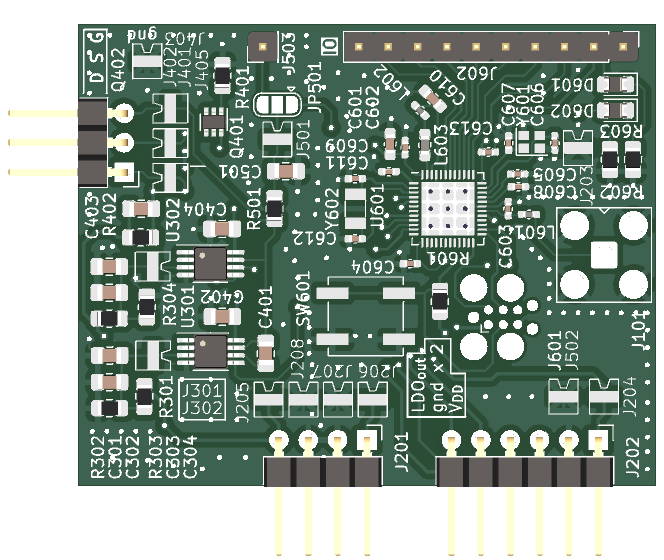
\includegraphics[width=\textwidth]{sensorBord}
        \caption{De ISFET uitlezende PCB.} 
        \label{fig:sensorPCB}
    \end{subfigure}
    \hfill
    \begin{subfigure}[b]{0.60\textwidth}
        \centering
        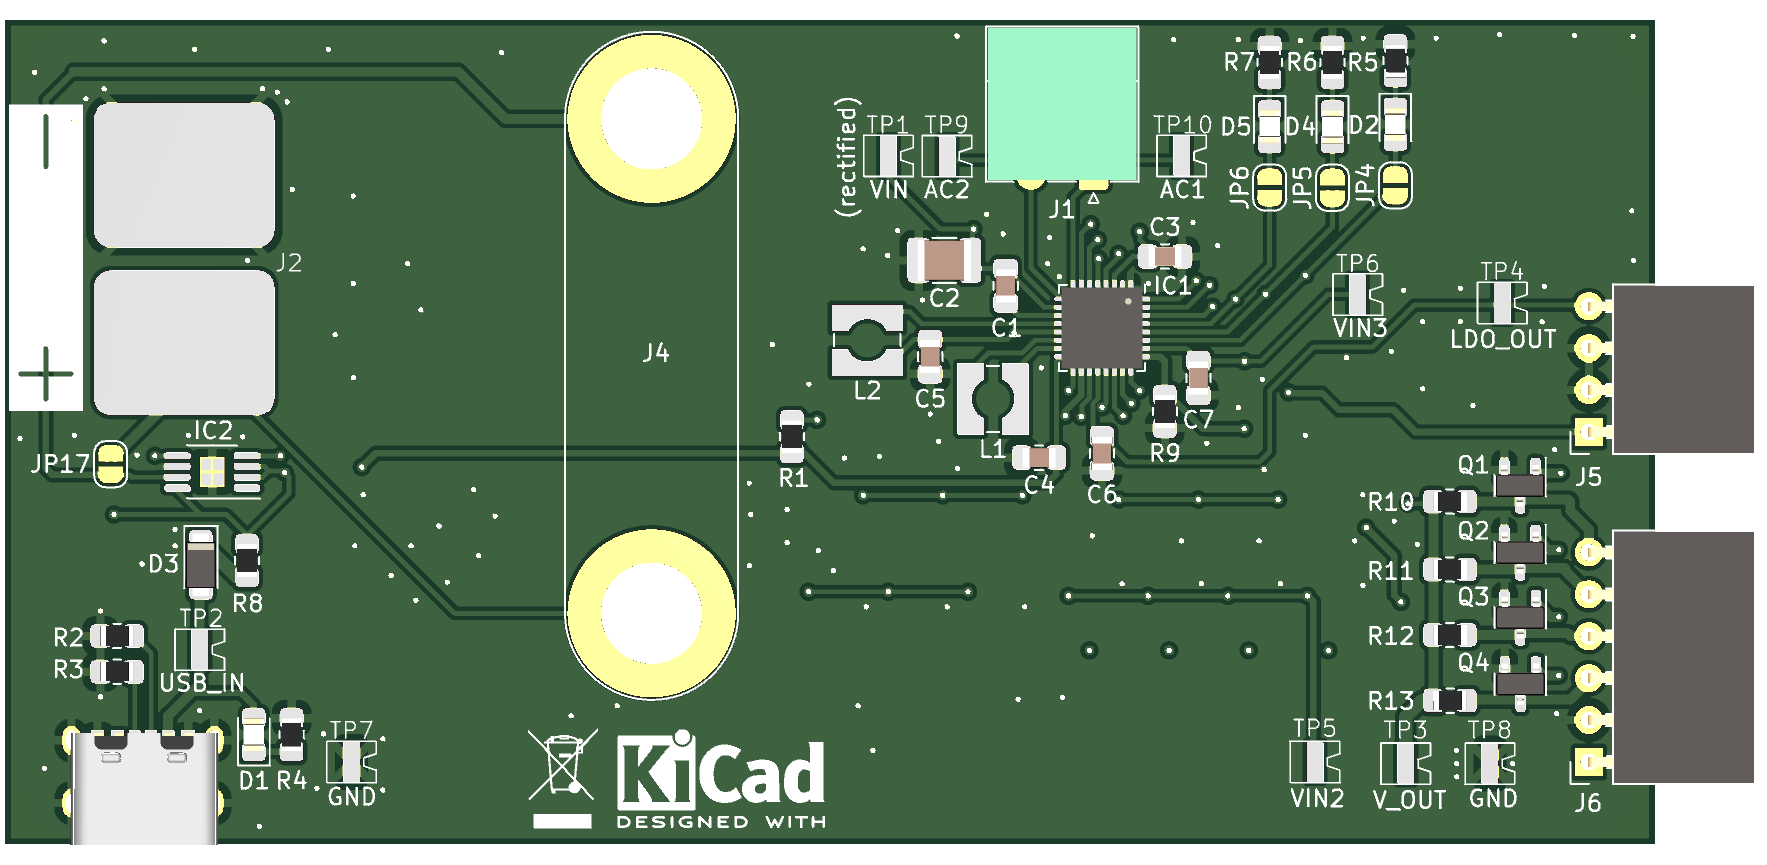
\includegraphics[width=\textwidth]{powerandharvest}
        \caption{De voeding en harvesting PCB.} 
        \label{fig:powerPCB}
    \end{subfigure}
    \caption{De gemaakte PCB's.}
    \label{fig:PCBs}
\end{figure}